En esta ocasión se debe encontrar, dada una serie de habitaciones, la forma menos costosa de unirlas, teniendo que derribar determinadas paredes para lograrlo. Las mismas poseen un costo en energía que va del cero al nueve.\\

Dada 2 habitaciones: el muro menos costoso a derribar que une a las mismas será la elección a tomar para formar la solución.

Tenemos que tener en cuenta que hay muros que no son derribables. Estos se representan con un numeral ('\#').

Para resolver este problema, caracterizaremos el mismo sobre un grafo que representa cada habitación como un conjunto de puntos caminables adyacentes entre si. Y a las paredes rompibles, es decir, las paredes numeradas como aristas entre los puntos caminables.\\
Las paredes irrompibles no conectarán habitaciones.\\

Lo que se busca entonces, es una forma de unir todas las habitaciones de la forma menos costosa. 

Para que exista solución, tiene que haber una forma de cruzar de una habitación a otra. Por lo tanto, tiene que existir una pared rompible que las una. La misma conectará dos puntos caminables, uno en cada habitación. 

Dentro de cada habitación, los  puntos caminables estarán unidos por aristas de valor nulo.

Una pared numerada tiene que unir exactamente dos puntos de izquierda a derecha o de arriba hacia abajo. Por lo tanto, las direcciones no utilizadas tienen que estar ocupadas por paredes, ya que si no, existe ambig{\"u}edad para determinar que puntos conecta.

Como en este problema no existen movimientos en diagonal sobre el mapa, los únicos casos válidos serán:

\vspace*{0.3cm} \vspace*{0.3cm}
  \begin{center}
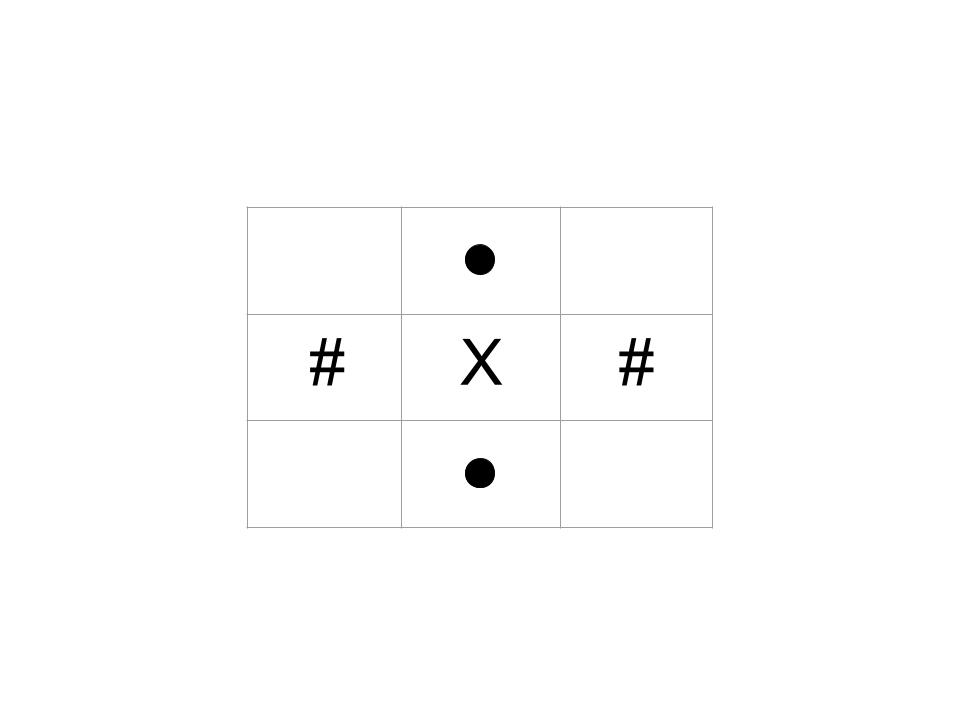
\includegraphics[scale=0.2]{./EJ2/casosValidos.jpg}
{}
  \end{center}
  \vspace*{0.3cm}

Y el simétrico.

Para obtener la soluci\'on, se busca el arbol generador mínimo (AGM) del grafo planteado mediante el algoritmo de Kruskal. 

A dicho AGM resultante del algoritmo se le calcula el esfuerzo total, que será la suma de todas las paredes destruidas para unir las habitaciones, es decir, la solución al problema planteado.\\

Para desarrollar el algoritmo de b\'usqueda del AGM del grafo, implementamos las funciones find y uni\'on, las cuales se encargan de ir armando el arbol avanzando dentro de una habitación o cruzando a otra habitación rompiendo una pared.
